\chapter{Hydrostatica}
\label{sec:Hydrostatica}

%%%%%%%%%%%%%%%%%%%%%%%%%%%%%%%%%%%%%%%%%%%%%%%%%%%%%%%%%%%%%%%%%%%%%%%%%%%%%%%%%%%%
	\section{Inleiding}
	\label{sec:Hydrostatica Inleiding}
In veel ingenieurstoepassingen komen situaties voor waar stilstaande fluïda interageren met een constructie. Het fluïdum zal ten gevolge van zijn gewicht bepaalde krachten uitoefenen op deze constructie. Het deel van de fluïdummecahnica waarin dit soort situaties bestudeerd wordt, wordt hydrostatica genoemd. In de komende secties zullen een aantal eenvoudige vergelijkingen voor het beschrijven van een stilstaand fluïdum besproken worden.

%%%%%%%%%%%%%%%%%%%%%%%%%%%%%%%%%%%%%%%%%%%%%%%%%%%%%%%%%%%%%%%%%%%%%%%%%%%%%%%%%%%%
	\section{Hydrostatische druk}
	\label{sec:Hydrostatische druk}
	
Beschouw een stilstaand fluïdum. We kunnen hieruit een balk met als grondvlak een rechthoekige driehoek afzonderen (Figuur \ref{sec:Hydrostatica}). Aangezien de volledige vloeistof in rust is zal ook de vloeistof binnen de balk in rust zijn en zullen er geen schuifspanningen aanwezig zijn (de snelheid is overal 0 dus is de snelheidsgradiënt ook overal 0). We kunnen nu een krachtenevenwicht schrijven voor dit elementje. In de richtingen loodrecht op de rechthoekszijden wordt dit:
\begin{eqnarray}
	F_A &=& F_C \cos(\alpha) \\
	F_B &=& F_C \sin(\alpha)
\end{eqnarray}
De uitgeoefende krachten zijn de resultante van een normaalspanning over de drie oppervlakken. Indien we het elementje klein genoeg kiezen zal deze spanning ook constant zijn over het oppervlak. Dus:
\begin{eqnarray}
	A \sigma_A &=& C \sigma_C \cos(\alpha) \\
	B \sigma_B &=& C \sigma_C \sin(\alpha)
	\label{eqn:druk_scalair_krachtenevenwicht}
\end{eqnarray}
Aangezien de driehoek rechthoekig is geldt ook dat:
\begin{eqnarray}
	A &=& C \cos(\alpha) 
	\label{eqn:druk_scalair_rechthoekige_driehoek1} \\
	B &=& C \sin(\alpha)
	\label{eqn:druk_scalair_rechthoekige_driehoek2}
\end{eqnarray}
Indien we de uitdrukkingen (\ref{eqn:druk_scalair_rechthoekige_driehoek1}) en (\ref{eqn:druk_scalair_rechthoekige_driehoek2}) in vullen in (\ref{eqn:druk_scalair_krachtenevenwicht}) bekomen we:
\begin{eqnarray}
	\sigma_A &=& \sigma_C \\
	\sigma_B &=& \sigma_C
	\label{eqn:druk_scalair}
\end{eqnarray}
Of de spanning op alle 3 de vlakken is dezelfde, onafhankelijk van de hoek van de driehoek. Het negatieve van deze spanning noemen we de hydrostatische druk $p$ met als eenheid [Pa] of [\unit{N/m^2}]. In ingenieurstoepassingen wordt ook vaak gewerkt met de eenheid [bar] ($1\unit{bar} = 100000\unit{Pa}$) of met de Engelse eenheid [psi] ($1\unit{psi} \approx 6895\unit{Pa}$). Volgens de meest gangbare conventies wordt deze in tegenstelling tot een normaalspanning positief gerekend indien ze werkt om het elementje te verkleinen. Aangezien de druk onafhankelijk is van de richting van het oppervlak waar ze op inwerkt is het een scalaire grootheid. Aangezien de druk een normaalspanning is zal ze ook steeds loodrecht op een oppervlak inwerken.
\begin{figure}[htb]
	\centering
	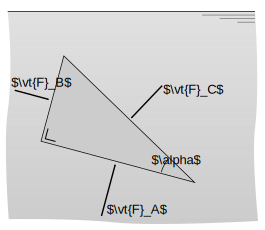
\includegraphics{fig/hydrostatica/driehoek_uit_stilstaande_vloeistof}
	\caption{Een driehoekig elementje afgezonderd uit een stilstaand fluïdum.}
	\label{fig:driehoek_uit_stilstaande_vloeistof}
\end{figure}

Beschouw nu een horizontaal oppervlak ondergedompeld in een stilstaand fluïdum. We kunnen de kracht die de vloeistof op \'e\'en zijde van het oppervlak uitoefent bepalen door opnieuw een geschikt deel van de vloeistof af te zonderen en er een krachten evenwicht op toe te passen. Zonderen we het deel af met als begrenzing het vrije vloeistof oppervlak, het beschouwde oppervlak en de verticalen vertrekkende vanaf de randen van het begrenzende oppervlak (Figuur \ref{fig:oppervlak_in_stilstaande_vloeistof}). Aangezien de vloeistof stilstaat werken er opnieuw geen schuifspanningen in op het afgezonderde deel. De enige inwerkende krachten zijn de zwaartekracht die inwerkt op de vloeistof en de reactiekracht van het oppervlak op de vloeistof.
\begin{figure}[htb]
	\centering
	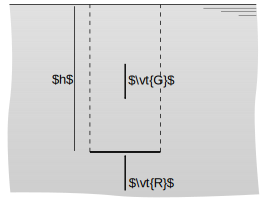
\includegraphics{fig/hydrostatica/oppervlak_in_stilstaande_vloeistof}
	\caption{Vlakke horizontale plaat oppervlak ondergedompeld in een stilstaand fluïdum.}
	\label{fig:oppervlak_in_stilstaande_vloeistof}
\end{figure}
\begin{equation}
	 R = G
\end{equation}
Indien we veronderstellen dat de dichtheid van het fluïdum onafhankelijk is van de positie in het fluïdum kunnen we het gewicht van het fluïdum berekenen door de dichtheid te vermenigvuldigen met de valversnelling en het beschouwde volume. De reactiekracht op het oppervlak moet opnieuw de resultante zijn van de druk. Indien we het oppervlak klein genoeg beschouwen wordt dit:
\begin{equation}
	 p \diff A = \rho g \diff A h
\end{equation}
of:
\begin{equation}
	 p = \rho g h
\end{equation}
Met andere woorden, de druk in het fluïdum is enkel afhankelijk van de verticale afstand tot het vrije oppervlak. In deze situatie hebben we de druk op het vrije vloeistof oppervlak verondersteld 0 te zijn. In de werkelijkheid zal ook hier een druk heersen, namelijk de druk veroorzaakt door de luchtlaag boven het vloeistof oppervlak, de atmosfeerdruk. Meer algemeen kunnen we het drukverschil tussen twee punten in een fluïdum met constante dichtheid bereken als:
\begin{equation}
	\Delta p = -\rho g \Delta z
\end{equation}

Indien de dichtheid (of de valversnelling) niet constant is dienen we een integraal te berekenen tussen de twee beschouwde punten. Dit wordt:
\begin{equation}
	\Delta p = -\int \rho g \diff z
\end{equation}
of
\begin{equation}
	\diff p = -\rho g \diff z
\end{equation}

De eerder gemaakte veronderstelling dat de druk aan het vrije vloeistof oppervlak 0 is in plaats van atmosfeerdruk is een vaak gebruikte veronderstelling in de ingenieurswetenschappen. Aangezien in veel toepassingen de atmosfeerdruk overal aanwezig is heeft ze vaak geen invloed op de berekening van krachten. Vaak wordt de druk dan ook weergegeven ten opzichte van de atmosfeerdruk. We noemen dit een overdruk (E: gauge pressure). De atmosfeerdruk heeft dus een overdruk van 0\unit{Pa}. Een overdruk van 1\unit{bar} betekent dat de druk 100 000\unit{Pa} hoger is dan de lokale atmosfeerdruk. Aangezien de atmosfeerdruk varieert in de tijd en met positie kunnen overdrukken gemeten op verschillende tijdstippen of locaties moeilijk met elkaar vergeleken worden. Wanneer we echter geïnteresseerd zijn in krachten die uitgeoefend worden door een fluïdum kunnen overdrukken wel vergeleken worden aangezien de atmosfeerdruk vaak geen rol speelt bij de berekening van krachten.


Een klassieke toepassing van hydrostatica is het meten van drukken met behulp van een U-buis manometer (Figuur \ref{fig:Ubuis_manometer}). Hierbij bevindt een vloeistof met hoge massadichtheid zich in een U vormige doorzichtige buis. E\'en zijde van de buis wordt verbonden met de zone waar de te meten druk heerst. De andere zijde wordt vaak verbonden met de vrije atmosfeer. Aangezien wanneer de dichtheid constant is de druk enkel varieert met de hoogte zal ter hoogte van de onderste stippellijn de druk in beide benen van de manometer gelijk zijn. Ter hoogte van de bovenste stippellijn zal er dus een drukverschil heersen gelijk aan het verschil van dichtheid van de twee fluïda vermenigvuldigd met de valversnelling en het hoogteverschil tussen de twee niveaus. De overdruk in het reservoir ter hoogte van de bovenste stippellijn kan dus berekend worden als: 
\begin{equation}
	p_{over} = p-p_{atm} = (\rho_m-\rho_f) g \Delta h
\end{equation}
\begin{figure}[htb]
	\centering
	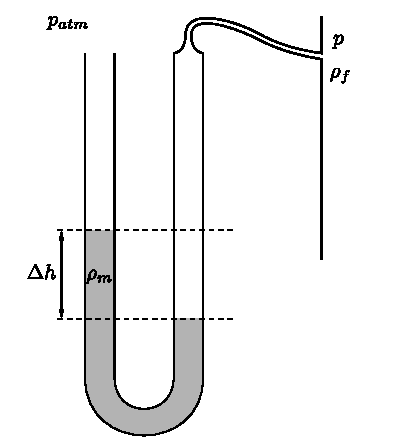
\includegraphics{fig/hydrostatica/U-buis_manometer}
	\caption{U-buis manometer.}
	\label{fig:Ubuis_manometer}
\end{figure}
Vroeger werd vaak kwik als meetvloeistof gebruikt omwille van zijn hoge dichtheid ($\rho_{Hg} \simeq 13600\unit{kg/m^3}$). Wanneer een kwikmanometer gebruikt wordt om de druk in een gas te meten kan vaak de dichtheid van het gas verwaarloosd worden. Dit is ook de herkomst van de eenheid voor druk [mm Hg] die overeenkomt met het hoogteverschil afgelezen tussen de 2 manometer benen uitgedrukt in mm.

Ander types analoge manometers (vb. zuiger-, bourdon- of membraanmanometers) maken gebruik van veren om een druk uit te lezen. Elektronische manometers kunnen gebruik maken van rekstrookjes, piëzo elementen of andere technieken om drukken te meten.

%%%%%%%%%%%%%%%%%%%%%%%%%%%%%%%%%%%%%%%%%%%%%%%%%%%%%%%%%%%%%%%%%%%%%%%%%%%%%%%%%%%%
	\section{Hydrostatische krachten}
	\label{sec:Hydrostatische krachten}

		\subsection{krachten op rechte oppervlakken}
Om de kracht die door een druk op een oppervlak wordt uitgeoefend te berekenen, dienen we de druk te vermenigvuldigen met het oppervlak waarop deze inwerkt. De richting waarin de kracht werkt komt overeen met de richting waarin de druk werkt, dus loodrecht op het oppervlak.
\begin{equation}
	F = p A
\end{equation}
Indien de druk over een oppervlak niet constant is kunnen we het oppervlak opdelen in verschillende delen en de krachten die op de verschillende delen werken optellen. In de limiet, wanneer de delen infinitesimaal klein worden, zal de druk op elk deeltje constant zijn. De som van de verschillende krachten wordt dan een integraal over het oppervlak.
\begin{equation}
	F = \int_A p \diff A
	\label{eqn:kracht op een recht oppervlak}
\end{equation}
of
\begin{equation}
	\diff F = p \diff A
\end{equation}
Deze uitdrukking kan ook grafisch weergegeven worden. Indien we de druk die heerst in een bepaald punt als hoogte uitzetten loodrecht op het oppervlak (Figuur \ref{fig:grafische_weergave_integraal}), dan zal de integraal (\ref{eqn:kracht op een recht oppervlak}) overeenkomen met het volume van de gevormde figuur.

\begin{figure}[htb]
	\centering
	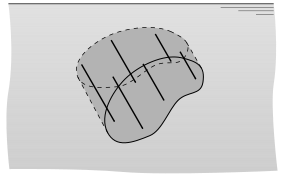
\includegraphics{fig/hydrostatica/grafische_weergave_integraal}
	\caption{Grafische weergave van de berekening van de kracht op een recht oppervlak.}
	\label{fig:grafische_weergave_integraal}
\end{figure}

De richting waarin de kracht werkt zal nog steeds gelijk zijn aan de richting waarin de druk werkt dus loodrecht op het oppervlak. Om de inwerkende kracht volledig te karakteriseren hebben we echter ook zijn aangrijpingspunt nodig. Voor het aangrijpingspunt van de kracht moet gelden dat het moment dat de kracht rond dit punt uitoefent 0 is. Het moment dat de kracht uitoefent is de som van de momenten die de infinitesimale krachten uitoefenen. In een cartesiaans assenstelsel wordt dit:
\begin{eqnarray}
	M_x &=& \int_A  p (y-y_z)  \diff A = 0 \\
	M_y &=& \int_A  p (x-x_z)  \diff A = 0
\end{eqnarray}
Indien we opnieuw de grafische voorstelling van hierboven gebruiken, dan komen de bovenstaande vergelijkingen overeen met de definitie van het zwaartepunt van het gevormde volume. Het aangrijpingspunt van de kracht komt dus overeen met het zwaartepunt van het volume gevormd door de druk als hoogte loodrecht op het oppervlak uit te zetten.

In het geval van hydrostatisch drukken leid dit vaak zeer eenvoudige uitdrukkingen voor de kracht en het aangrijpingspunt aangezien de druk lineair verloopt met de diepte.

\begin{voorbeeld}
	\label{vb:luik}
	Bepaal de grootte en het aangrijpingspunt van de resulterende kracht op het luik ondergedompeld in een fluïdum met dichtheid $\rho$ getoond in de figuur. De bovenzijde bevindt zich op een diepte $d$, het luik heeft een hoogte $h$ en breedte $b$ (de breedte staat loodrecht op het vlak van de figuur).
	\begin{center}
		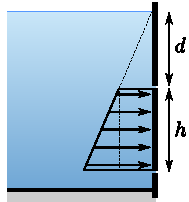
\includegraphics{fig/hydrostatica/kracht_op_luik}
	\end{center}
	Boven het fluïdum en aan de achterzijde van het luik heersen atmosfeerdruk. We kunnen deze dus buiten beschouwing laten aangezien ze netto geen kracht uitoefent op het luik. De druk binnen de vloeistof verloop linear zoals aangegeven op de figuur. Deze grootte van de kracht is dus gelijk aan het volume van de figuur gevormd door de druk uit te zetten op een verticaal vlak, dit het volume van een balk met een trapezium als grondvlak en lengte $b$. Het grondvlak van de figuur kan opnieuw opgesplitst worden in een rechthoek en een rechthoekige driehoek. Beide hebben dezelfde basis $h$. De hoogte van de rechthoek komt overeen met de druk aan het bovenste punt van het luik, $\rho g d$. de hoogte van de driehoek komt overeen met het drukverschil tussen het bovenste en onderste punt van het luik, $\rho g h$ De grootte van de kracht wordt dan:
	\begin{align*}
		F &= \left( A_{\text{rechthoek}} + A_{\text{driehoek}} \right) b\\
		  &= \left( \rho g d h + 1/2 \rho g h h \right) b
	\end{align*}

	Om het aangrijpingspunt te bepalen zoeken we de hoogte van het zwaartepunt van de figuur. Dit kunnen we bepalen als het gewogen gemiddelde van het zwaartepunt van de rechthoek en de driehoek, gewogen met hun oppervlaktes:
	\begin{equation*}
		y_z = \frac{ y_{z,\text{rechthoek}} A_{\text{rechthoek}} + y_{z,\text{driehoek}} A_{\text{driehoek}}}{A_{\text{rechthoek}} + A_{\text{driehoek}}}
	\end{equation*}
	Aangezien het zwaartepunt van de rechthoek op $1/2 h$ van de onderzijde ligt en dat van de driehoek op $1/3 h$ wordt de afstand van het aangrijpingspunt tot de onderzijde:
	\begin{align*}
		y_z &= \frac{ 1/2 h \rho g d h + 1/3 h 1/2 \rho g h h}{\rho g d h + 1/2 \rho g h h} \\
		    &= \frac{ 1/2 d h + 1/6 h^2}{d + 1/2 h}
	\end{align*}
\end{voorbeeld}

		\subsection{krachten op gebogen oppervlakken}
Wanneer we te maken hebben met gebogen oppervlakken zal het bepalen van de resultante krachten vaak niet meer zo eenvoudig zijn. Aangezien de druk steeds loodrecht op een oppervlak inwerkt, moeten we hier ook rekening houden met de richting van het oppervlak om de kracht in een bepaalde richting te berekenen. Beschouw als voorbeeld het oppervlak in Figuur \ref{fig:kracht_gebogen_oppervlak}. Beschouwen we een infinitesimaal deel van dit oppervlak met oppervlakte $\diff A$. Op dit deel werkt een kracht $\diff F$ ten gevolge van de hydrostatische druk $p$ in de richting loodrecht op het oppervlak met als grootte:
\begin{equation}
	\diff F = p \diff A
\end{equation}
Met behulp van de normaalvector op het oppervlak kunnen we de kracht vector schrijven als (vectoren zullen in deze cursus in het vet aangeduid worden.):
\begin{equation}
	\vt{\diff F} = -p \vt{n} \diff A
\end{equation}
\begin{figure}[htb]
	\centering
	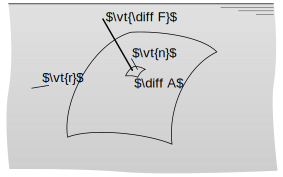
\includegraphics{fig/hydrostatica/kracht_gebogen_oppervlak}
	\caption{Kracht op een infinitesimaal stukje van een gebogen oppervlak.}
	\label{fig:kracht_gebogen_oppervlak}
\end{figure}
Indien we nu de kracht willen berekenen die in een bepaalde richting (volgens een vector $\vt{r}$) wordt uitgeoefend op het oppervlak kunnen we de kracht op het infinitesimaal oppervlak projecteren in de gewenste richting. Met behulp van het inwendig product van vectoren wordt dit:
\begin{equation}
	\diff F_r = -p \vt{n} \cdot \vt{r} \diff A
\end{equation}
De totale kracht kunnen we opnieuw berekenen door te integreren over het volledige oppervlak:
\begin{equation}
	F_r = \int_A -p \vt{n} \cdot \vt{r} \diff A
\end{equation}
Hierin zullen de normaalvector en de druk in veel gevallen afhankelijk zijn van de positie. Om de integraal uit te werken zullen dus afhankelijk van de situatie geschikte uitdrukkingen voor $p$ en $\vt{n}$ moeten opgesteld worden.

Voor horizontale krachten kan de uitwerking van bovenstaande integraal vermeden worden. Het is namelijk steeds mogelijk een volume af te zonderen met als begrenzingen het beschouwde oppervlak, een projectie van dit oppervlak op een verticaal vlak loodrecht op de beschouwde richting en de verbinding tussen de twee. Ook voor dit volume moet een krachtenevenwicht gelden. In de horizontale richting werken er slechts twee krachten, aan de ene zijde de reactie kracht van het beschouwde oppervlak op het volume, en aan de andere zijde de hydrostatische kracht ten gevolge van het aangrenzende fluïdum. Deze krachten zijn dus gelijk en aangezien het tweede oppervlak een recht oppervlak is, bovendien een verticaal oppervlak, kan de kracht, en het aangrijpingspunt, berekend worden volgens de formules voor een recht oppervlak. De horizontale kracht op eender welk oppervlak is dus gelijk aan de kracht die inwerkt op de projectie van het oppervlak op een verticaal vlak dat loodrecht staat op de beschouwde richting. Ook het aangrijpingspunt (in elk geval de hoogte van het aangrijpingspunt) van de kracht kan volgend de formules en eenvoudige methodes voor vlakke oppervlakken berekend worden. Dit wordt voor een geval in 2 dimensies geïllustreerd in Figuur \ref{fig:kracht_gebogen_oppervlak_vereenvoudigd_2d}.

Ook voor verticale krachten kan de berekening vereenvoudigd worden. De kracht op zal namelijk gelijk zijn aan het gewicht van het volume boven het oppervlak alsof dit volledig met vloeistof gevuld zou zijn. Dit komt echter overeen met de berekening van een volume met een gekromd eindvlak. Hiervoor zal vaak een volume integraal uitgewerkt moeten worden wat de berekening niet steeds vereenvoudigd. Ook hier zal het aangrijpingspunt van de kracht samenvallen met het zwaartepunt van het beschouwde volume (Figuur \ref{fig:kracht_gebogen_oppervlak_vereenvoudigd_2d}).
\begin{figure}[htb]
	\centering
	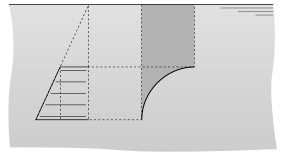
\includegraphics{fig/hydrostatica/kracht_gebogen_oppervlak_vereenvoudigd_2d}
	\caption{Vereenvoudigde berekening van krachten op een gebogen oppervlak.}
	\label{fig:kracht_gebogen_oppervlak_vereenvoudigd_2d}
\end{figure}

Het feit dat de kracht op een oppervlak in een stilstaande vloeistof onafhankelijk is van het totale volume vloeistof in het reservoir leidt soms tot verwarring. Bekijk als voorbeeld Figuur \ref{fig:hydrostatische_paradox}. Ter hoogte van de onderste stippellijn zal voor alle vormen van reservoir de druk gelijk zijn. Aangezien ook de oppervlakte gelijk is zal ook de kracht die inwerkt op het oppervlak gelijk zijn. Dit is onafhankelijk van de hoeveelheid massa in het reservoir of dat er daadwerkelijk massa zich boven het oppervlak bevindt. Dit wordt vaak de hydrostatische paradox genoemd.
\begin{figure}[htb]
	\centering
	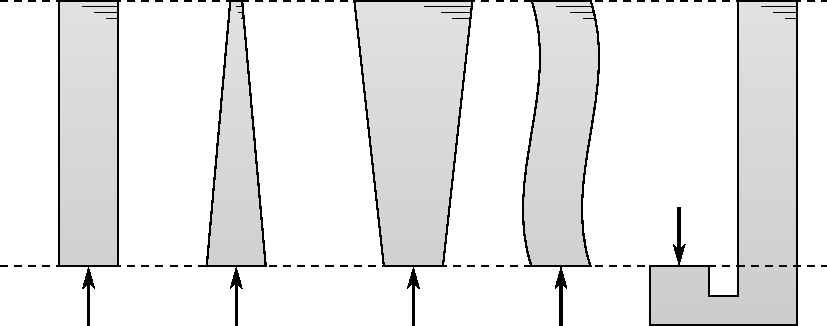
\includegraphics{fig/hydrostatica/hydrostatische_paradox}
	\caption{Een voorbeeld van de hydrostatische paradox.}
	\label{fig:hydrostatische_paradox}
\end{figure}

\begin{voorbeeld}
	Bereken de horiontale en vertikale kracht die uitgeoefend wordt op een kwart van een cilindermantel met straal $r$ en breedte $b$ waarvan het bovenste punt zich op een diepte $d$ bevindt zoals afgebeeld in Figuur \ref{fig:kracht_gebogen_oppervlak_vereenvoudigd_2d}.

	Het horizontale gedeelte van de kracht zal gelijk zijn aan de horizontale kracht uitgeoefend op een verticaal vlak met dezelfde geprojecteerde oppervlakte en kan dus zoals in Voorbeeld \ref{vb:luik} berekend worden:
	\begin{align*}
		F_{hor} &= \left( A_{\text{rechthoek}} + A_{\text{driehoek}} \right) b\\
		        &= \left( \rho g d r + 1/2 \rho g r r \right) b \\
		y_z &= \frac{ y_{z,\text{rechthoek}} A_{\text{rechthoek}} + y_{z,\text{driehoek}} A_{\text{driehoek}}}{A_{\text{rechthoek}} + A_{\text{driehoek}}} \\
		    &= \frac{ 1/2 d r + 1/6 r^2}{d + 1/2 r}
	\end{align*}

	Om de verticale kracht te berekenen moeten we het volume boven het oppervlak berekenen (het donkere gedeelte op de figuur). Het gewicht van dit volume water komt overeen met de verticale kracht. Bemerk dat het volume niet noodzakelijk gevuld met water moet zijn. Het volume is eenvoudig te berekenen al de oppervlakte van een rechthoek min de oppervlakte van de kwart cilinder vermenigvuldigd met de lengte:
	\begin{align*}
		F_{ver} &= \rho g (A_{\text{rechthoek}} - \frac{1}{4}A_{\text{cilinder}}) L\\
		        &= \rho g \left( (d+r)r - \frac{1}{4} \pi r^2 \right) b
	\end{align*}

	Het aangrijpingspunt van de verticale kracht kan op dezelfde manier gevonden worden als dat van de horizontale component, enkel moet het zwaartepunt van de kwart cirkel berekend worden. Dit ligt op $\frac{4r}{3\pi}$ van het middelpunt. De verdere uitwerking verloopt analoog als hierboven.
\end{voorbeeld}

	\section{Drijven en stabiliteit}
Wanneer een schip te water gelaten wordt zal het net zo diep in het water zakken totdat de resultante van de drukkrachten uitgeoefend door het water op de romp van het schip gelijk is aan het gewicht van het schip (Figuur \ref{fig:opwaartse_kracht}). De resultante van deze drukkrachten kunnen we berekenen met behulp van de vereenvoudigde methode voor verticale krachten zoals hierboven uitgewerkt en wordt vaak de opwaartse kracht of Archimedeskracht genoemd. Wanneer een voorwerp volledig ondergedompeld is moeten zowel de drukkrachten aan de onderzijde als aan de bovenzijde in rekening gebracht worden. De opwaartse kracht is echter steeds gelijk aan de valversnelling vermenigvuldigd met de verplaatste massa fluïdum.
\begin{equation}
	F_{opwaarts} = \rho_{\text{fluïdum}} g V_{\text{verplaatst}}
\end{equation}
Deze vergelijking wordt ook vaak de wet van Archimedes genoemd naar de Griekse wiskundige.
\begin{figure}[htb]
	\centering
	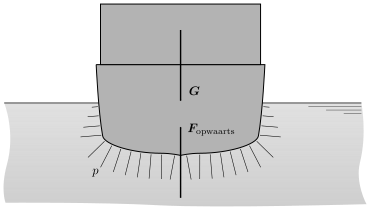
\includegraphics{fig/hydrostatica/opwaartse_kracht}
	\caption{De opwaartse kracht uitgeoefend op de romp van een schip ten gevolge van de hydrostatische druk.}
	\label{fig:opwaartse_kracht}
\end{figure}

Opdat een voorwerp zou kunnen drijven dient zijn massa kleiner te zijn dan de massa water die het kan verplaatsen.

Bij het ontwerp van de romp van schepen dient er steeds voor gezorgd te worden dat het schip in zekere mate rol stabiel is. Met andere woorden dat het schip geen slagzij zal maken. Wanneer het aangrijpingspunt van de opwaartse kracht of het drukkingspunt (E: centre of buoyancy) hoger gelegen is dan het zwaartepunt van het schip is dit steeds gegarandeerd. Wanneer het schip een uitwijking ondervindt (bijvoorbeeld ten gevolge van golfslag) zal het vanzelf terugkeren naar de evenwichtspositie. In de meeste gevallen zal het drukkingspunt echter lager gelegen zijn dan het zwaartepunt (Figuur \ref{fig:opwaartse_kracht}). De stabiliteit is nu niet meer gegarandeerd. De romp dient nu zo ontworpen te worden dat wanneer het schip een uitwijking aanneemt het drukkingspunt zich verder verplaatst dan het zwaartepunt. Op deze manier ontstaat er een terugwerkend moment dat het schip terug naar de evenwichtspositie zal brengen. Vanaf een bepaalde initiële uitwijking zal het drukpunt echter minder opgeschoven zijn dan het zwaartepunt. Wanneer het schip verder dan deze hoek rolt ontstaat er een meewerkend koppel en zal het schip kapseizen.